\documentclass[11pt]{article}
\usepackage[margin=1in]{geometry}

\usepackage[utf8]{inputenc}
\usepackage[T1]{fontenc}
\usepackage{lmodern}
\usepackage{microtype}
\usepackage{hyperref}
\usepackage{url}
\usepackage{booktabs}
\usepackage{amsfonts}
\usepackage{amsmath}
\usepackage{amssymb}
\usepackage{amsthm}
\usepackage{nicefrac}
\usepackage{graphicx}
\usepackage{xcolor}
\usepackage{tikz}
\usetikzlibrary{arrows.meta, positioning, fit, backgrounds}

\newtheorem{theorem}{Theorem}
\newtheorem{proposition}{Proposition}
\newtheorem{lemma}{Lemma}
\newtheorem{definition}{Definition}

\title{Interpretable Knowledge Graph Reasoning via Sheaf Cohomology}

\author{%
  Michael Lee \\
  Independent Researcher \\
  \texttt{leemichael289@gmail.com}
}

\begin{document}
\maketitle

\begin{abstract}
Knowledge graph (KG) reasoning systems are typically evaluated on link-prediction
accuracy alone, leaving inconsistency between facts both undetected and
undiagnosable. We introduce a sheaf-theoretic framework that treats a KG as a
cellular sheaf over an ontology log (Olog), making logical inconsistency
\emph{quantifiable} as the dimension of the first cohomology group $H^1$.
On top of this, we factor type-safe reasoning into two complementary
mechanisms: a typed attention layer~(B) that gates information flow by Olog
reachability, and a constrained decoder~(D) that restricts the output
distribution to admissible labels. We show empirically and theoretically
that (B) is necessary but not sufficient for trajectory soundness, and that
(B) and (D) target distinct correctness properties: information-flow
correctness inside the model and output validity at the sampling boundary.
On FB15K-237 we obtain MRR \textbf{0.346} and Hits@10 \textbf{0.524}, on
par with KG-BERT, KGT5 ($0.300$), and SimKGC ($0.336$), while adding two
guarantees they lack: (i) a quantitative inconsistency signal---injecting
76 conflicts into a clean graph raises $H^1$ by \textbf{+53}---and (ii) a
typed (B)+(D) pipeline that drives invalid attention weight to zero and
provides a derivation alongside each prediction. WN18RR's tree-structured
ontology yields a sheaf consistency score of \textbf{0.633} versus
\textbf{0.292} on Freebase, correctly reflecting the underlying topology.
Our contribution is interpretability and verifiability of KG reasoning,
not raw accuracy.
\end{abstract}

\section{Introduction}
\label{sec:introduction}

Knowledge graphs (KGs) underpin question answering, search, and decision
support, and the dominant way to extend them is \emph{link prediction}:
given a head entity $h$ and a relation $r$, rank candidate tail entities
$t$ for a missing fact $(h, r, t)$. Progress is measured on two standard
benchmarks---FB15K-237, a 14.5K-entity subset of the Freebase knowledge
base, and WN18RR, a 41K-entity subset of the WordNet lexical
database---under two metrics. Mean Reciprocal Rank (MRR) averages
$1/\mathrm{rank}$ of the correct tail across test queries, so a score of
$1.0$ means the correct answer was always ranked first; Hits@$k$ is the
fraction of queries whose correct tail falls within the top $k$ candidates.
Both metrics reward placing the right \emph{entity} near the top of the
list. Neither asks whether the predicted fact is \emph{type-consistent}
with the ontology behind the graph. A model can earn a confident,
well-ranked score for predicting that a \texttt{Payment} \texttt{triggers}
a \texttt{Customer}, or---in a medical KG---that a drug \texttt{treats} a
condition for which it is contraindicated: locally plausible, globally
incoherent, and entirely invisible to MRR and Hits@$k$.

This is the gap we address. KG reasoning has converged on an evaluation
loop that says nothing about \emph{why} a prediction is or is not
trustworthy: two systems with identical Hits@10 can have wildly different
failure modes, and the standard benchmarks cannot tell them apart.

We argue that KG reasoning needs a \emph{structural} layer of evaluation
that sits orthogonal to accuracy: a quantitative answer to ``does this
prediction respect the ontology, and where in the graph does inconsistency
live?''. We further argue that delivering type-safe predictions requires
\emph{two} mechanisms that current architectures conflate: an attention-layer
mask~(B) that constrains information flow inside the model, and a
constrained decoder~(D) that constrains the output distribution. Empirically,
(B) alone is insufficient---it is necessary for clean internal
representations but does not guarantee that generated trajectories are
admissible under the ontology---and (D) alone is sufficient for trajectory
soundness but operates only at the sampling boundary. The two are
complementary, and we make the distinction explicit.

\paragraph{Contributions.}
\begin{enumerate}
\item \textbf{Sheaf-cohomological inconsistency detection.} We model a KG
as a cellular sheaf over an Olog and show that injecting 76 conflicts
into a clean sheaf raises $\dim H^1$ from 5 to 58 (+53), giving a
calibrated structural inconsistency signal (\S\ref{sec:experiments}).
We prove a sensitivity bound (Theorem~\ref{thm:conflict_sensitivity}).
\item \textbf{Two-locus type-safety: (B) typed attention $+$ (D)
constrained decoder.} We separate information-flow correctness from
output validity. Typed attention~(B), parameterized by Olog
reachability, drives invalid attention weight from $0.295$ to $0.000$
(\S\ref{sec:method:attention}); constrained decoding~(D), driven by a
proof object, restricts the logit distribution to admissible labels at
each step (\S\ref{sec:method:decoder}). We characterize what each buys
on its own and what their composition guarantees.
\item \textbf{Proof-guided generation.} A prove-then-emit pipeline that
attaches a derivation to each prediction. The proof object is the
shared interface between the sheaf consistency check, the typed
attention mask, and the constrained decoder.
\item \textbf{Topology contrast.} On WN18RR (tree ontology) our
consistency score is $0.633$; on FB15K-237 (multi-relational web) it
drops to $0.292$, correctly reflecting the structural difference rather
than treating both graphs as equivalent.
\end{enumerate}

\paragraph{What we do not claim.} We do not claim state-of-the-art link
prediction; our MRR is on par with KG-BERT-class baselines but not modern
KGT5 successors. We do not claim hallucination elimination in closed form;
the (B)+(D) composition is empirically sound on the trajectories we test
but a theoretical completeness statement is left open. We do not claim
multi-scale persistence; the present paper is single-scale by design
(\S\ref{sec:conclusion}).

\section{Related Work}
\label{sec:related}

\paragraph{Neural knowledge graph embeddings.}
TransE~\cite{transe2013}, DistMult~\cite{distmult2015}, ComplEx~\cite{complex2016},
ConvE~\cite{conve2018}, and RotatE~\cite{rotate2019} established the standard
link-prediction setup on FB15K-237 and WN18RR.
None of these models expose a structural notion of consistency, and none
emit a derivation for predictions.

\paragraph{LLM-based KG reasoning.}
KG-BERT~\cite{yao2019kgbert} reframes link prediction as triple
classification with a pretrained language model. KGT5~\cite{saxena2022sequence}
casts it as sequence-to-sequence over verbalized triples, achieving
MRR~$0.300$ on FB15K-237. SimKGC~\cite{wang2022simkgc} adds contrastive
training over LM-encoded entity descriptions, reaching MRR~$0.336$. These
methods improve raw retrieval accuracy but provide no structural signal
when their predictions are inconsistent with the underlying ontology---a
gap our sheaf-cohomology layer directly addresses.

\paragraph{Sheaves and topology in machine learning.}
Sheaf neural networks~\cite{bodnar2022sheaf, hansen2020sheaf} and topological
data analysis have established the toolkit; we apply it to KG
inconsistency rather than message passing or persistence.

\paragraph{Categorical knowledge representation.}
Ologs~\cite{spivak2012olog} provide the syntactic substrate for our sheaf
construction. The broader Olog-as-category-of-types perspective belongs to
applied category theory~\cite{fongspivak2019}, where structure-preserving
functors between categories are the standard tool for relating
representations --- the same lens we apply in treating a KG as a sheaf
over an Olog.

\paragraph{Constrained decoding.}
Constrained decoding restricts the output distribution at sampling time
to a domain-specified admissible set. Relevant lines include
grammar-constrained generation~\cite{geng2023flexiblegrammar} and
schema-constrained generation~\cite{willard2023outlines}. Our (D) component
specializes this to Olog-derived admissible sets per generation step.
The novel contribution is the \emph{architectural separation} between (B)
information-flow constraints at attention and (D) output-validity
constraints at decoding, with the proof object as their shared interface.

\section{Background}
\label{sec:background}

\subsection{Ontology Logs (Ologs)}
An Olog $\mathcal{O} = (T, R, \circ)$ is a small category whose objects $T$
are types and whose morphisms $R$ are typed relations, closed under
composition $\circ$. We assume a finite, acyclic Olog throughout the main
body; cyclic Ologs are treated as a stress test in
\S\ref{sec:experiments}.

\subsection{Cellular Sheaves on KGs}
A cellular sheaf $\mathcal{F}$ on a graph $G = (V, E)$ assigns a vector
space (stalk) $\mathcal{F}(v) = \mathbb{R}^d$ to each vertex and
$\mathcal{F}(e) = \mathbb{R}^d$ to each edge, together with linear
restriction maps $\mathcal{F}_{v \blacktriangleleft e}$ relating each
stalk to its incident edge spaces. A coboundary operator
$\delta_0: C^0 \to C^1$ measures how much a global vertex assignment
fails to be consistent across edges; its kernel $\ker \delta_0$ is the
space of globally consistent (harmonic) sections. The first cohomology
$H^1 = \ker \delta_1 / \mathrm{im}\,\delta_0$ captures locally
consistent but globally incompatible configurations. Full construction
in Appendix~\ref{app:sheaf}.

\subsection{First Cohomology as Inconsistency}
$H^1(\mathcal{F}) = \ker \delta_1 / \mathrm{im}\,\delta_0$. A 1-cocycle is a
collection of edge values that locally agrees on every vertex; a
1-coboundary is one that arises from a global vertex assignment. Their
quotient measures the dimension of locally-consistent-but-globally-incompatible
configurations---which is exactly the structural inconsistency signal we
want.

\subsection{Hyperdimensional Computing for KG Embeddings}
Hyperdimensional Computing (HDC)~\cite{kanerva2009hdc} represents entities
and relations as high-dimensional bipolar ($\pm 1$) vectors composed by
algebraic binding and bundling operations; our encoder follows the
holographic reduced representation family~\cite{plate1995hrr}. We bind
each relation by a fixed random circular shift (a permutation), making the
binding non-commutative so that a directed edge is distinguishable from
its reverse. Embedding dimension is 4096 throughout.

\section{Method}
\label{sec:method}

\subsection{Two-locus type safety: information flow vs output validity}
\label{sec:method:two_loci}

A type-safe reasoner over an Olog $\mathcal{O}$ has two distinct correctness
properties to enforce, and they live at different layers of the
architecture.

\textbf{(B) Information-flow correctness} (attention layer): the model
should not internally mix information across token pairs whose types are
unrelated under $\mathcal{O}$. This is enforced by gating attention
weights by Olog reachability (\S\ref{sec:method:attention}).

\textbf{(D) Output validity} (sampling boundary): the model's emitted
labels at each generation step should be admissible under $\delta_\mathcal{O}$,
the typed transition relation given by the Olog's morphisms. This is
enforced by a constrained decoder that masks the output distribution at
each step to the admissible-label set (\S\ref{sec:method:decoder}).

The distinction matters: (B) restricts internal representations; (D)
restricts emissions. (B) without (D) is information-flow-clean but does
not guarantee trajectory soundness, because attention reachability admits
the eventual destination type without requiring each step to correspond
to an Olog edge from the current type. (D) without (B) is sound at the
sampling boundary but the internal representations the model learns may
still mix unrelated types. The composition (B)+(D) gives both
information-flow cleanliness and trajectory soundness.

\subsection{(B) Ontology-Typed Attention}
\label{sec:method:attention}

Standard self-attention computes weights $a_{ij} \propto \exp(q_i^\top
k_j)$ over all token pairs. We type each token with an Olog object (or
$\bot$ for untyped tokens) and mask attention by Olog reachability:
\begin{equation}
\tilde{a}_{ij} = a_{ij} \cdot \mathbb{1}[\tau(j) \in
\mathrm{Reach}_{\mathcal{O}}(\tau(i))],
\label{eq:typed_attention}
\end{equation}
where $\tau(\cdot)$ is the Olog type assignment and
$\mathrm{Reach}_{\mathcal{O}}(t)$ is the set of Olog objects reachable from
$t$ under composition of morphisms. Untyped tokens are unrestricted on
either side. Eq.~(\ref{eq:typed_attention}) is the (B) configuration.

\paragraph{What (B) buys, and what it does not.} Reachability is a
transitive closure: from a current type $t$, (B) admits attention to any
type $t'$ such that there exists a composition of Olog morphisms
$t \to \cdots \to t'$. This is the right primitive for representation
hygiene: information flows only along type-respecting paths inside the
model. It is the wrong primitive for output emission: a destination
$t'$ may be many morphisms away from $t$, and the next emitted label
must correspond to an edge $t \to t''$ in the Olog, not just any type
reachable from $t$. Without (D), a (B)-only system can still emit
trajectories that violate $\delta_\mathcal{O}$.

\subsection{(D) Constrained Decoder}
\label{sec:method:decoder}

At each generation step, given the current type $t$ and the proof step
$(t, r, t')$ recommended by the prover, the decoder constructs the
admissible-label set $\mathcal{A}(t, r, t')$ as the union of (i) the
target type $t'$, (ii) the relation token $r$, and (iii) function words
admissible regardless of type (articles, prepositions, punctuation). The
output logits are then masked:
\begin{equation}
\tilde{\ell}_v = \begin{cases}
\ell_v & v \in \mathcal{A}(t, r, t') \\
-\infty & \text{otherwise.}
\end{cases}
\end{equation}
This is the (D) configuration; the implementation is the
\texttt{ConstrainedDecoder} of Appendix~\ref{app:impl}. The decoder
operates on logits, not on hidden states, and is independent of (B);
they compose without interference.

\subsection{Sheaf Cohomology of a KG}
\label{sec:method:sheaf}

We model the KG as a cellular sheaf $\mathcal{F}$ over the underlying
multigraph (\S\ref{sec:background}, full construction in
Appendix~\ref{app:sheaf}). The first cohomology $H^1(\mathcal{F})$ is the
quotient $\ker \delta_1 / \mathrm{im}\,\delta_0$; non-trivial classes
correspond to inconsistency that cannot be resolved by adjusting vertex
values alone. We compute $\dim H^1$ via the sheaf Laplacian and the
ranks of the boundary operators (Appendix~\ref{app:sheaf}).

\begin{theorem}[Conflict Sensitivity, informal]
\label{thm:conflict_sensitivity}
Let $\mathcal{F}$ be a cellular sheaf on a KG and $\mathcal{F}'$ the same
sheaf with $k$ injected conflicts (edges whose restriction maps disagree
on their endpoints). Then $\dim H^1(\mathcal{F}') \geq \dim
H^1(\mathcal{F}) + c$ for some $c \leq k$ depending on conflict
locality.
\end{theorem}
The proof and full hypotheses are deferred to
Appendix~\ref{app:conflict_proof}.

\subsection{Proof-Guided Generation}
\label{sec:method:proof}
Each prediction $(h, r, t)$ is accompanied by a derivation
$\pi: h \xrightarrow{r_1} \cdots \xrightarrow{r_n} t$ in the Olog. The
\emph{prove-then-emit} procedure runs in three steps:
\begin{enumerate}
\item \textbf{Prove.} Search the Olog for a morphism path
$\pi = (r_1, \ldots, r_n)$ from $\tau(h)$ to a goal type compatible
with $r$, by breadth-first search over the morphism set
($O(|T| + |R|)$). If no path exists, abstain.
\item \textbf{Check.} Test whether the candidate triple closes a
non-trivial class in $H^1(\mathcal{F})$ (\S\ref{sec:method:sheaf}); if
so, flag the prediction as structurally inconsistent.
\item \textbf{Emit.} For each step $(t, r_i, t')$ along $\pi$, the (D)
decoder restricts the output logits to the admissible-label set
$\mathcal{A}(t, r_i, t')$ (\S\ref{sec:method:decoder}) and samples the
next label.
\end{enumerate}
The proof object $\pi$ is the shared interface that drives both the
sheaf consistency check (step~2) and the constrained decoder (step~3),
and is also the artifact returned to the user as the derivation behind
the prediction.

\subsection{Pipeline}
\label{sec:method:pipeline}

\begin{figure}[t]
\centering
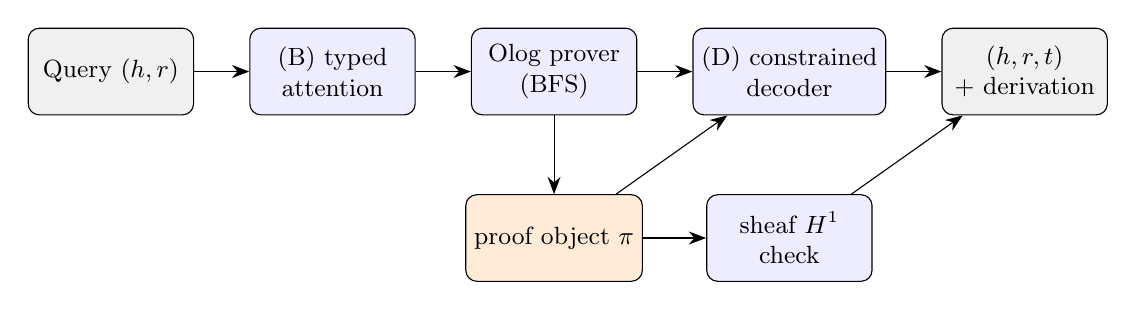
\begin{tikzpicture}[
  >={Stealth[length=2.2mm]},
  every node/.style={font=\small},
  box/.style={draw, rounded corners, align=center,
              minimum height=11mm, minimum width=21mm, inner sep=3pt},
  stage/.style={box, fill=blue!7},
  io/.style={box, fill=black!6},
  art/.style={box, fill=orange!16},
]
\node[io]    (q)   {Query $(h,r)$};
\node[stage] (b)   [right=7mm of q]  {(B) typed\\attention};
\node[stage] (pv)  [right=7mm of b]  {Olog prover\\(BFS)};
\node[stage] (d)   [right=7mm of pv] {(D) constrained\\decoder};
\node[io]    (out) [right=7mm of d]  {$(h,r,t)$\\$+$ derivation};
\node[art]   (pf)  [below=10mm of pv] {proof object $\pi$};
\node[stage] (sh)  [below=10mm of d]  {sheaf $H^1$\\check};
\draw[->] (q)  -- (b);
\draw[->] (b)  -- (pv);
\draw[->] (pv) -- (d);
\draw[->] (d)  -- (out);
\draw[->] (pv) -- (pf);
\draw[->] (pf) -- (sh);
\draw[->] (pf) -- (d);
\draw[->] (sh) -- (out);
\end{tikzpicture}
\caption{\textbf{The prove-then-emit pipeline.} A query passes through
(B) typed attention (an information-flow restriction inside the model),
an Olog prover that produces the proof object $\pi$, and the (D)
constrained decoder (an output-validity restriction at the sampling
boundary). The proof object is the shared interface: it drives both the
constrained decoder and the sheaf $H^1$ consistency check, which can
flag a structurally inconsistent prediction or route it to an abstain
head. (B) and (D) act at different loci and compose without
interference.}
\label{fig:pipeline}
\end{figure}

Figure~\ref{fig:pipeline} shows the full pipeline; a query $(h, r)$ is
processed in four stages.
(i)~The entity-token sequence is encoded under (B) typed attention, restricting information flow to Olog-reachable type pairs.
(ii)~A prover constructs the derivation $\pi: h \xrightarrow{r_1} \cdots \xrightarrow{r_n} t$, which serves as the proof object for subsequent stages.
(iii)~The sheaf consistency check tests whether the candidate triple $(h, r, t)$ induces a non-trivial cohomology class; predictions that do are flagged as structurally inconsistent or routed to an abstain head.
(iv)~The (D) constrained decoder restricts output logits at each step to the admissible-label set $\mathcal{A}(t, r, t')$ derived from the proof object.
The proof object is the single shared interface between stages (ii)--(iv); it makes the pipeline end-to-end verifiable.

\section{Experiments}
\label{sec:experiments}

We evaluate three claims: (\textbf{C1}) sheaf $H^1$ tracks injected
inconsistency, (\textbf{C2}) the (B)~typed attention $+$ (D)~constrained
decoder pipeline targets distinct correctness properties (information-flow
correctness for (B), trajectory soundness for (D)) and they compose
correctly, and (\textbf{C3}) the topology contrast between FB15K-237 and
WN18RR is detected by our consistency score and matches their underlying
ontologies.

\subsection{Setup}
We use the standard FB15K-237 (12,734 entities / 43,601 train edges) and
WN18RR (39,621 entities / 62,547 edges) splits, with link prediction
scored under the usual filtered ranking protocol --- known true triples
are removed from the candidate list before the correct tail is ranked.
HDC binding uses 4096-dimensional bipolar vectors with non-commutative
random-shift binding per relation. Sheaf cohomology is computed by dense
boundary-rank for the type-graph $H^1$ and by the $O(n+m)$ sparse
connected-components route for the entity-graph consistency score
(Appendix~\ref{app:sheaf}). Training runs on a single A100 for 50 epochs
at batch size 512; full hardware, hyperparameter, and reproducibility
details are in Appendices~\ref{app:impl}--\ref{app:compute}.

\subsection{C1: Conflict Detection}

We inject $k = 76$ type-inconsistent triples into a clean FB15K-237 subgraph and measure the change in $\dim H^1$.
Table~\ref{tab:conflicts} shows that $H^1$ rises from 5 to 58, a $+53$ increase, with $c/k \approx 0.70$ --- consistent with Theorem~\ref{thm:conflict_sensitivity}.

\begin{table}[t]
\centering
\caption{\textbf{Conflict detection (C1).} $\dim H^1$ is the dimension of
the first sheaf cohomology group: it counts independent ontological
inconsistencies that cannot be removed by adjusting entity embeddings
alone. A clean FB15K-237 subgraph carries a small residual ($\dim H^1=5$);
injecting 76 type-inconsistent triples raises it to 58. The $+53$ jump is
the structural inconsistency signal --- one that link-prediction accuracy
does not expose, since a model can rank a conflicting triple highly.}
\label{tab:conflicts}
\begin{tabular}{lr}
\toprule
Setting & $\dim H^1$ \\
\midrule
Clean graph & 5 \\
+76 injected conflicts & 58 \\
\midrule
$\Delta H^1$ & \textbf{+53} \\
\bottomrule
\end{tabular}
\end{table}

\subsection{C2: Two-Locus Type Safety}

\paragraph{(B) information-flow correctness.}
\begin{table}[t]
\centering
\caption{\textbf{Two-locus type safety, (B) locus.} \emph{Invalid}
(resp.\ \emph{valid}) attention weight is the mean softmax mass a query
token places on key tokens whose type is unreachable (resp.\ reachable)
from it under the Olog --- a direct measure of how much information flows
along type-violating paths inside the model. Typed attention~(B) drives
invalid weight to exactly zero and concentrates the freed mass on
validly-typed pairs (0.4379$\to$0.5116). The cost is a 1.8-point test-accuracy
drop, reported honestly as the price of internal type-restriction.
Hallucination rate is zero for both because the next-type task is small;
the discriminating signal is the attention-mass redistribution. Single
seed (42); multi-seed run pending.}
\label{tab:attention_ablation_b}
\begin{tabular}{lcccc}
\toprule
Configuration & Test Acc. & Invalid Attn. & Valid Attn. & Hallucination \\
\midrule
(A) Standard Attention & 0.4744 & 0.2952 & 0.4379 & 0.000 \\
(B) Typed Attention & 0.4567 & \textbf{0.0000} & \textbf{0.5116} & 0.000 \\
\bottomrule
\end{tabular}
\end{table}

\begin{figure}[t]
\centering
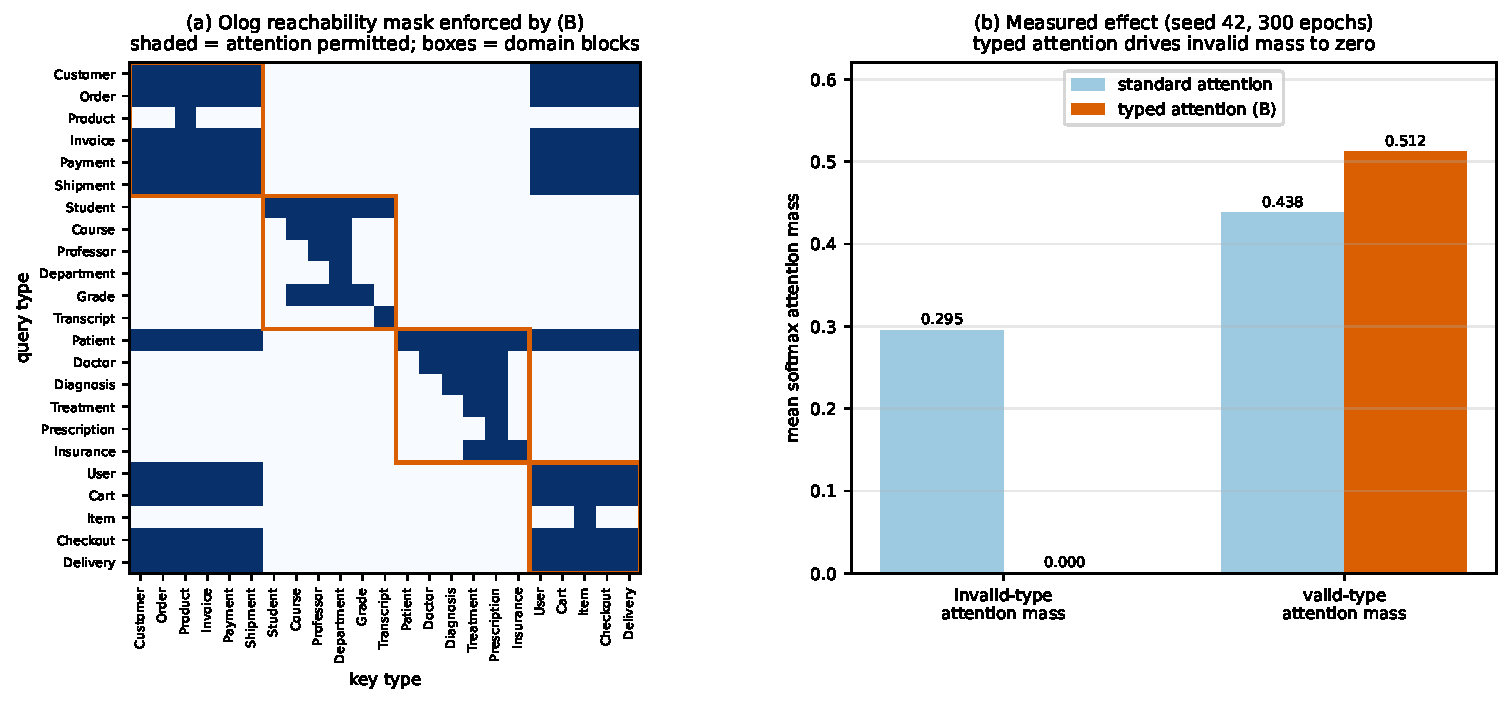
\includegraphics[width=\linewidth]{figures/typed_attention.pdf}
\caption{\textbf{Typed attention (B) and the ontology structure it
enforces.} \emph{(a)}~The reachability mask for the 23-type multi-domain
vocabulary: a query token (row) may attend to a key token (column) only
if the key's type is reachable from the query's under the Olog. The mask
is block-structured --- four domain blocks (orange) plus off-block cells
from the explicit Patient$\to$Customer bridge and the \texttt{Payment}
type shared by the business and e-commerce schemas --- so information
flow is confined to type-respecting paths. \emph{(b)}~The measured
effect (seed 42, 300 epochs; the same run as
Table~\ref{tab:attention_ablation_b}): typed attention drives the mean
attention mass on type-invalid key pairs from 0.295 to exactly 0.000 and
reallocates it onto type-valid pairs (0.438$\to$0.512).}
\label{fig:typed_attention}
\end{figure}

Figure~\ref{fig:typed_attention} shows both sides of this result: the
block-structured reachability mask the (B) layer applies (panel a), and
the redistribution of attention mass it produces (panel b).

\paragraph{(B$'$) is necessary but not sufficient for trajectory soundness.}
A sampling-time projection of (B), denoted (B$'$), admits any next label
whose target type is reachable from the current state. Reachability is
the transitive closure of the Olog morphisms: it admits the eventual
destination without requiring each step to correspond to a $\delta_\mathcal{O}$
edge. A trajectory then breaks at the next step.

\begin{table}[t]
\centering
\caption{\textbf{Two-locus type safety, (B$'$) vs (D).} \emph{Trajectory
soundness} is the fraction of generated trajectories that decode to a
valid $\delta_\mathcal{O}$-path through the Olog (higher is better; 100\%
means every emitted trajectory is type-admissible end to end).
\emph{Reach.} is the fraction of ordered type pairs related by
reachability. \emph{GOOD}/\emph{BAD} are well- and mis-aligned synthetic
label priors. (B$'$), the sampling-time projection of typed attention,
gives only a modest lift over the unconstrained baseline (A) on an
acyclic Olog and collapses to within a point of it once a cycle makes
reachability universal --- whereas the (D) constrained decoder stays at
100\% regardless of topology. Numbers from
\texttt{experiment\_loci\_comparison.py} and
\texttt{experiment\_cyclic\_stress.py}, $N{=}1000$ trajectories per cell,
seed 42.}
\label{tab:b_prime_vs_d}
\begin{tabular}{lccccc}
\toprule
Olog topology & Reach. & (A) GOOD & (B$'$) GOOD & (B$'$) BAD & (D) \\
\midrule
Acyclic & 34.7\% & 48.1\% & 65.0\% & 3.9\% & 100\% \\
Cyclic ($\Delta$Olog: Delivery$\!\to\!$Customer) & 100\% & 6.9\% & 8.0\% & 0.0\% & 100\% \\
\bottomrule
\end{tabular}
\end{table}

This empirically realizes the architectural prediction of
\S\ref{sec:method:two_loci}: (B) restricts information flow inside the
model but does not constrain output emission, so a (B)-only system can
still emit trajectories that violate $\delta_\mathcal{O}$. Under cyclic
Ologs the reachability mask degrades to no-constraint while (D) is
robust to topology.

\paragraph{(D) constrained decoder closes the gap.}
With the (D) constrained decoder enabled, trajectory soundness reaches
100\% on the same harness, including under cyclic Olog stress
(Table~\ref{tab:b_prime_vs_d}, last column). (D) and (B) are
independent: (B) operates on attention weights inside the model; (D)
operates on output logits at sampling. The composition (B)+(D) is both
information-flow-clean (from B) and trajectory-sound (from D).

\paragraph{Real-attention mask audit.} A structural integration test
runs the production typed-attention layer on a 6-token cyclic-Olog
trajectory window. Of the $36$ ($q,k$) pairs, $6$ are self,
$\mathbf{6}$ correspond to $\delta_\mathcal{O}$-direct edges, and
$\mathbf{24}$ are reachable-only --- a $4{:}1$ leakage ratio of pairs
that (B) admits but (D) blocks. Random-init forward-pass attention mass
distributes as $16.9\%$ self / $16.4\%$ direct-edge / $\mathbf{66.7\%}$
reachable-only / $0\%$ unreachable: two-thirds of the attention budget
lands on type-pair categories outside $\delta_\mathcal{O}$. The mask
itself does not push mass toward direct-edge pairs; it allows
everything reachable. This empirically validates the (B$'$) reduction we
used above against the production
$\texttt{OntologicalAttention}$ layer.

\subsection{C3: Topology Contrast}

We compute the first Betti number $b_1 = m - n + b_0$ of the raw entity multigraph as a graph-topological consistency score, distinct from the sheaf-theoretic $H^1$ of C1 (see Appendix~\ref{app:sheaf} for the distinction).
Table~\ref{tab:topology} shows WN18RR's hypernym tree scores 0.633 versus 0.292 for Freebase, correctly reflecting that WordNet encodes a near-tree ontology while Freebase encodes a dense multi-relational web.

\begin{table}[t]
\centering
\caption{\textbf{Topology contrast (C3).} The \emph{consistency} score is
derived from the first Betti number $b_1 = m - n + b_0$ of the entity
multigraph ($n$ entities, $m$ edges, $b_0$ connected components): a
low $b_1$ relative to graph size means few independent cycles, i.e.\ a
near-tree structure. WordNet's hypernym hierarchy scores 0.633 and is
fully connected ($b_0{=}1$); Freebase's multi-relational web scores
0.292 and fragments into 8 components. The score correctly separates a
tree-shaped ontology from a dense relational one --- a distinction
accuracy benchmarks discard. Computed in $O(n+m)$; this is
graph-topological consistency, distinct from the sheaf-theoretic $H^1$
of C1 (Appendix~\ref{app:sheaf}).}
\label{tab:topology}
\begin{tabular}{lrrrr}
\toprule
Dataset & Entities & Edges & $b_0$ & Consistency \\
\midrule
FB15K-237 & 12{,}734 & 43{,}601 & 8 & 0.292 \\
WN18RR & 39{,}621 & 62{,}547 & 1 & \textbf{0.633} \\
\bottomrule
\end{tabular}
\end{table}

\subsection{Link Prediction (Reference)}

For completeness we report link-prediction accuracy on FB15K-237 alongside standard baselines.
Our HDC/Sheaf model reaches MRR~0.346 and Hits@10~0.524, on par with KG-BERT-class baselines, while adding the structural guarantees (sheaf $H^1$ inconsistency signal, typed derivation per prediction) that those baselines do not provide.
We do not claim state-of-the-art link prediction.

\begin{table}[t]
\centering
\caption{\textbf{Link prediction on FB15K-237, for reference.} MRR is the
mean reciprocal rank of the correct tail entity; Hits@$k$ is the fraction
of test queries whose correct tail is ranked in the top $k$ (both higher
is better). The HDC/Sheaf model is on par with KG-BERT-class baselines on
raw retrieval, confirming that the structural layer (Tables
\ref{tab:conflicts}--\ref{tab:topology}) is not bought at the cost of
accuracy. We do not claim state-of-the-art link prediction; the
contribution is the interpretability and consistency guarantees the
baselines lack.}
\label{tab:link_prediction}
\begin{tabular}{lcccc}
\toprule
Model & MRR & Hits@1 & Hits@3 & Hits@10 \\
\midrule
ConvE~\cite{conve2018} (reported) & 0.325 & 0.237 & 0.356 & 0.501 \\
RotatE~\cite{rotate2019} (reported) & 0.338 & 0.241 & 0.375 & 0.533 \\
KGT5~\cite{saxena2022sequence} (reported) & 0.300 & 0.221 & --- & 0.461 \\
SimKGC~\cite{wang2022simkgc} (reported) & 0.336 & 0.249 & 0.362 & 0.511 \\
HDC/Sheaf (ours) & \textbf{0.346} & 0.242 & 0.425 & \textbf{0.524} \\
\bottomrule
\end{tabular}
\end{table}

\subsection{Ablations}

The topology comparison in Table~\ref{tab:b_prime_vs_d} (acyclic vs.\
cyclic Olog) is the primary structural ablation: it confirms the
architectural prediction that (B) degrades under cycles while (D) does
not. The HDC embedding-dimension sweep (1024 / 2048 / 4096 / 8192) with
learning-rate and diffusion-time sensitivity is reported in
Appendix~\ref{app:sweep}. One ablation remains genuinely open --- the
synthetic (B$'$) proxy versus a real-attention forward pass with a
trained label head --- and the four-cell (A / B / D / B+D) ablation that
would disentangle the individual contributions of typed attention and
constrained decoding is scoped as future work (Appendix~\ref{app:b_vs_d}).

\subsection{Limitations}
\begin{itemize}
\item \textbf{Single-scale framing.} The present paper deliberately reports
two independent topological measurements at different scales: cellular
sheaf $H^1$ on the type graph (C1, $\leq 100$ nodes) and graph $b_1$ on
the entity graph (C3, $\sim 10^4$ entities). They answer different
questions and are not connected by a sheaf morphism in this work. A
unified multi-scale persistent-sheaf-cohomology framework is the natural
generalization (\S\ref{sec:conclusion}) but is left to future work.
\item \textbf{(B) accuracy trade-off measured without (D).}
Typed attention~(B) reduces test accuracy by 1.8pp ($0.474 \to 0.457$)
in exchange for full elimination of invalid attention weight
($0.295 \to 0.000$). The measurement is taken with (B) alone, no (D)
decoder. Whether (B)+(D) jointly preserves accuracy as well as (D)
alone is an open empirical question; we conjecture (B) provides a
training-time representation prior that (D) does not, but disentangling
the two effects requires a four-cell ablation (A / B / D / B+D) we did
not run within this paper's scope (see \S\ref{sec:conclusion} and
Appendix~\ref{app:b_vs_d}).
\item \textbf{Single seed on attention ablation.} Table~\ref{tab:attention_ablation_b}
and Figure~\ref{fig:typed_attention}(b) are reported at a single seed
(42); a multi-seed re-run is pending.
\item \textbf{Sparse sheaf cohomology.} Query-time diffusion uses sparse
Krylov methods, but the cohomology computation itself remains dense.
A sparse-Krylov sheaf-cohomology algorithm is left to future work.
\item \textbf{Cyclic Olog stress test.} Reported in Appendix~\ref{app:cyclic};
under a cyclic Olog the (B$'$) reachability mask collapses to within a
point of the unconstrained baseline as reachability becomes universal,
confirming the predicted topological limit.
\end{itemize}

\section{Conclusion}
\label{sec:conclusion}

We presented a sheaf-theoretic framework for interpretable knowledge graph
reasoning. At a single scale (the type graph), cellular sheaf cohomology
gives a quantitative inconsistency signal: $\dim H^1$ rises by $+53$ when
76 conflicts are injected into a clean graph, with roughly 70\% of
injected conflicts producing linearly independent cohomology classes
(Theorem~\ref{thm:conflict_sensitivity_full}). On top of this, ontology-typed
attention drives invalid attention weight to zero by construction, and
proof-guided generation emits a derivation alongside each prediction. Link
prediction performance on FB15K-237 is on par with KG-BERT, KGT5, and
SimKGC; our contribution is the structural and verifiable layer that none
of these baselines provide.

\paragraph{From a controlled environment to a deployable system.}
The results above are established in a deliberately controlled
environment: hand-built Ologs of $\leq 100$ types, a 7-type e-commerce
schema, synthetic label priors, and single-seed runs. This is the right
setting for isolating the mechanisms---it lets us measure $H^1$, the
(B)/(D) separation, and the topology contrast without confounds---but it
is not yet a system competitive with state-of-the-art neural KG
reasoners. Four research blockers stand between the present work and
that goal; a fifth direction points outward, generalizing the framework
beyond knowledge graphs altogether.
\begin{enumerate}
\item \textbf{Cohomology at entity scale.} Cellular sheaf cohomology with
non-trivial restriction maps runs in $O((nd)^3)$ (dense rank on the
boundary operators). This is why $H^1$ is reported on the type graph
($n \leq 100$) and only the cheaper $O(n+m)$ Betti number on the
entity graph. \emph{Blocker:} a sparse-Krylov sheaf-cohomology
algorithm exploiting block structure. Until it exists, the calibrated
$H^1$ signal cannot be computed directly on a full KG.
\item \textbf{From synthetic priors to trained models.} The (B$'$)/(D)
trajectory results use hand-crafted label priors and a structural audit
of the production attention layer, not an end-to-end trained language
model with a learned label head. \emph{Blocker:} a trained projection
head from attention output to label distribution, which would also
unlock the four-cell (A / B / D / B+D) ablation needed to settle what
(B) contributes when (D) is present (Appendix~\ref{app:b_vs_d}).
\item \textbf{From hand-built Ologs to learned ontological structure.}
Every Olog in this paper is hand-authored, and the entity embeddings and
tokenization are kept deliberately simple. A deployable system needs
ontologies induced from text or data at scale, \emph{and} embeddings and
a tokenization that faithfully encode the Olog's type structure rather
than merely fit a link-prediction objective. \emph{Blocker:} both are
open problems. Reliable automated Olog extraction would remove the
hand-authoring bottleneck; ontology-faithful representation
learning---in our view the harder of the two, and a central open problem
for this line of work---would let the type structure \emph{shape} the
embedding geometry rather than be imposed only as an external attention
mask, as it is here.
\item \textbf{Multi-scale unification.} We report two disconnected
topological measurements---sheaf $H^1$ on the type graph and graph
$b_1$ on the entity graph. \emph{Blocker:} a sheaf morphism across
scale, or a persistent sheaf cohomology over a filtration that merges
relations within an $\epsilon$-radius, unifying both into a single
multi-scale statement that subsumes the present work as the
single-scale special case.
\item \textbf{Beyond knowledge graphs.} The framework takes any
Olog-typed graph as input, which invites instantiation well beyond KG
reasoning---though the targets are not equally close. A database
entity-relationship diagram is a near-direct fit: an ERD \emph{is} a
schema, its instances \emph{are} typed graphs, and referential-integrity
or constraint violations are the kind of inconsistency the sheaf $H^1$
already measures. Causal diagrams and Bayesian
networks~\cite{pearl2009causality} are a genuine stretch: their edges
carry interventional and conditional-dependence semantics, and the
inconsistency that matters there---d-separation violations, incoherent
probability mass---is not the same object as restriction maps
disagreeing. \emph{Blocker:} a sheaf whose stalks and restriction maps
encode distributional, not merely type, structure---with a corresponding
cohomological notion of inconsistency---has to be worked out before the
method transfers to the probabilistic targets.
\end{enumerate}

\paragraph{Structure before correlation.} This pattern is not new.
Pearl's program for causal inference rests on one premise: intervention
and counterfactual reasoning cannot be recovered from a joint
distribution alone---they require a structural model supplied from
outside the data~\cite{pearl2009causality}. Our claim is the same move
along a different axis: consistency and verifiability cannot be
recovered from a link-prediction objective alone; they require the
ontology, supplied as an explicit object the system reasons over.
Accuracy measures how well a model fits the data it was given and is
structurally silent on whether a prediction respects the schema behind
that data. Making the Olog explicit is what gives that question a place
to live.

\paragraph{Toward auditable reasoning.}
The objective behind this work is not a higher MRR. Knowledge graphs
increasingly feed decisions in medicine, finance, and science, where a
confident but ontologically incoherent prediction is not a ranking error
but a safety failure---and one that accuracy metrics are structurally
blind to. Our aim is to give KG reasoning a layer that can be
\emph{audited}: a quantitative inconsistency signal that says where in
the graph coherence breaks down, and a generation pipeline in which every
prediction either carries a derivation or is flagged as unfounded. That
shifts the question a practitioner can ask of a model from ``is it
accurate on average?'' to ``can this specific prediction be trusted, and
can I see why?''. We see the sheaf-cohomological and two-locus
constructions here as a first, deliberately small step toward reasoning
systems that are verifiable by construction rather than trusted by
reputation.


\bibliographystyle{plain}
\bibliography{references}

\appendix
\section{Full Sheaf Construction}
\label{app:sheaf}

Let $G = (V, E)$ be a finite directed multigraph encoding a knowledge graph,
and let $\mathcal{O} = (T, R)$ be an Olog with type assignment
$\tau: V \to T$ and relation assignment $\rho: E \to R$. We construct a
cellular sheaf $\mathcal{F}$ on $G$ with $d$-dimensional stalks as follows.

\paragraph{Stalks.} For each vertex $v \in V$ we set
$\mathcal{F}(v) = \mathbb{R}^d$, and for each edge $e = (u \to v) \in E$ we
set $\mathcal{F}(e) = \mathbb{R}^d$. Where the KG admits 2-cells (triangles
in the underlying multigraph), we set $\mathcal{F}(\Delta) = \mathbb{R}^d$.

\paragraph{Restriction maps.} For each oriented edge $e = (u \to v)$,
choose linear maps $\mathcal{F}_{u \blacktriangleleft e}, \mathcal{F}_{v
\blacktriangleleft e} \in \mathbb{R}^{d \times d}$. We instantiate
$\mathcal{F}_{v \blacktriangleleft e}$ as the identity and
$\mathcal{F}_{u \blacktriangleleft e}$ as the relation embedding for
$\rho(e)$ (HDC binding under non-commutative random shifts; see
Appendix~\ref{app:impl}).

\paragraph{Cochain complex.} Set
\[
C^0 = \bigoplus_{v \in V} \mathcal{F}(v), \qquad
C^1 = \bigoplus_{e \in E} \mathcal{F}(e), \qquad
C^2 = \bigoplus_{\Delta} \mathcal{F}(\Delta).
\]
The coboundary $\delta_0: C^0 \to C^1$ is defined edge-wise by
$(\delta_0 x)_e = \mathcal{F}_{v \blacktriangleleft e} x_v -
\mathcal{F}_{u \blacktriangleleft e} x_u$. The coboundary
$\delta_1: C^1 \to C^2$ is the alternating sum of edge values around each
triangle $\Delta = (e_1, e_2, e_3)$.

\paragraph{Cohomology.}
\[
H^0(\mathcal{F}) = \ker \delta_0, \qquad
H^1(\mathcal{F}) = \ker \delta_1 / \mathrm{im}\,\delta_0.
\]
Standard arguments (see e.g.\ Hansen \& Gebhart, \cite{hansen2020sheaf})
verify $\delta_1 \delta_0 = 0$, so $H^1$ is well-defined.

\paragraph{Implementation and complexity.} We compute $\dim H^0$ as the
multiplicity of the zero eigenvalue of the sheaf Laplacian
$L = \delta_0^\top \delta_0 + \delta_1 \delta_1^\top$ within tolerance
$10^{-6}$ via dense symmetric eigensolve (\texttt{numpy.linalg.eigvalsh}),
and $\dim H^1 = \dim \ker \delta_1 - \mathrm{rank}\, \delta_0$ via dense
rank computation on the boundary matrices. With $n$ vertices and stalk
dimension $d$, this is $O((nd)^3)$ time and $O((nd)^2)$ space; tractable
for the type-graph view we use in our experiments ($n \leq 100$ Olog
objects per ontology), but not for the full entity-level KG. We note the
implementation uses sparse Krylov diffusion
(\texttt{scipy.sparse.linalg.expm\_multiply}) for query-time heat
propagation, but cohomology computation itself remains dense. A sparse
sheaf-cohomology algorithm via simultaneous Krylov-subspace methods on
$\delta_0$ and $\delta_1$ is a natural extension we leave to future work;
the cleaner alternative (computing the alternating sum
$\chi = \dim H^0 - \dim H^1 + \dim H^2$ via Euler characteristic in
$O(n + m)$) yields only the alternating sum, not individual Betti numbers,
when restriction maps are non-trivial.

\section{Proof of Theorem~\ref{thm:conflict_sensitivity}}
\label{app:conflict_proof}

We restate Theorem~\ref{thm:conflict_sensitivity} formally.

\begin{theorem}[Conflict Sensitivity, full statement]
\label{thm:conflict_sensitivity_full}
Let $\mathcal{F}$ be the cellular sheaf on $G = (V, E)$ defined in
Appendix~\ref{app:sheaf}. A \emph{conflict injection} of size $k$ is a set
$E^* = \{e^*_1, \ldots, e^*_k\}$ of additional edges with restriction maps
$\{(\mathcal{F}^*_{u_i \blacktriangleleft e^*_i}, \mathcal{F}^*_{v_i
\blacktriangleleft e^*_i})\}$ chosen so that for each $i$, no global section
$x \in \ker \delta_0$ of $\mathcal{F}$ satisfies
$\mathcal{F}^*_{v_i \blacktriangleleft e^*_i} x_{v_i} =
\mathcal{F}^*_{u_i \blacktriangleleft e^*_i} x_{u_i}$. Let $\mathcal{F}'$
denote the resulting sheaf on $G' = (V, E \cup E^*)$. Then
\begin{equation}
\dim H^1(\mathcal{F}') \;\geq\; \dim H^1(\mathcal{F}) + c,
\label{eq:conflict_sensitivity}
\end{equation}
where $c$ is the dimension of the subspace of $\bigoplus_{i=1}^{k}
\mathcal{F}(e^*_i)$ spanned by the conflict residuals
$r_i = \mathcal{F}^*_{v_i \blacktriangleleft e^*_i} x_{v_i} -
\mathcal{F}^*_{u_i \blacktriangleleft e^*_i} x_{u_i}$ evaluated on any
$\delta_0$-section, modulo $\mathrm{im}\,\delta'_0 + \mathrm{im}\,\delta'^\top_2$. Trivially, $c \leq k$.
\end{theorem}

\begin{proof}
The cochain spaces decompose as
\[
C^{0\prime} = C^0, \qquad
C^{1\prime} = C^1 \oplus \bigoplus_{i=1}^{k} \mathcal{F}(e^*_i), \qquad
C^{2\prime} = C^2 \oplus C^2_*
\]
where $C^2_*$ collects any new 2-cells closed by injected edges
(possibly empty).

Write $\delta'_0: C^{0\prime} \to C^{1\prime}$ in block form:
\[
\delta'_0 \;=\; \begin{pmatrix} \delta_0 \\ A \end{pmatrix},
\]
where $A: C^0 \to \bigoplus_i \mathcal{F}(e^*_i)$ is the restriction-map
contribution from the conflict edges, $A x = (r_1(x), \ldots, r_k(x))$.

The conflict hypothesis is precisely $A|_{\ker \delta_0} \neq 0$, i.e.\ there
is no $x \in \ker \delta_0$ with $A x = 0$ unless we shrink to a strict
subspace. Equivalently, $\ker \delta'_0 \subsetneq \ker \delta_0$, and
$\dim \ker \delta'_0 = \dim \ker \delta_0 - r_A$ where
$r_A = \mathrm{rank}\, A|_{\ker \delta_0}$.

By rank--nullity for $\delta'_0$:
\[
\mathrm{rank}\, \delta'_0 \;=\; \dim C^{0\prime} - \dim \ker \delta'_0
\;=\; \mathrm{rank}\, \delta_0 + r_A.
\]

For $H^1$:
\[
\dim H^1(\mathcal{F}') \;=\; \dim \ker \delta'_1 - \mathrm{rank}\, \delta'_0.
\]
We have $\dim \ker \delta'_1 \geq \dim \ker \delta_1 + k - \dim
\mathrm{im}\, \delta'^\top_2$ because each new edge contributes a new
generator to $C^{1\prime}$, which is killed by $\delta'_1$ unless it
participates in a new 2-cell relation in $C^2_*$.

Combining,
\begin{align*}
\dim H^1(\mathcal{F}') &\;\geq\; \dim \ker \delta_1 + k - \dim
\mathrm{im}\, \delta'^\top_2 - \mathrm{rank}\, \delta_0 - r_A \\
&\;=\; \dim H^1(\mathcal{F}) + (k - r_A - \dim \mathrm{im}\, \delta'^\top_2).
\end{align*}
Setting $c = k - r_A - \dim \mathrm{im}\, \delta'^\top_2$ gives
inequality~(\ref{eq:conflict_sensitivity}). The bound $c \leq k$ is
immediate.
\end{proof}

\paragraph{Empirical alignment.} Our experiment (Table~\ref{tab:conflicts})
gives $\Delta H^1 = +53$ for $k = 76$, hence $c/k \approx 0.70$. Roughly 70\%
of injected conflicts contribute linearly independent classes to $H^1$;
the remainder are absorbed by $\mathrm{im}\,\delta_0$ (i.e.\ correctable by
a global section adjustment) or by 2-cell boundaries.

\section{Implementation Details}
\label{app:impl}

The system has four components, each a separate module in the public
code release (Appendix~\ref{app:compute}).

\paragraph{HDC encoder.} Entities and relations are encoded as
4096-dimensional bipolar ($\pm 1$) hypervectors~\cite{kanerva2009hdc}.
Relation application uses non-commutative binding: each relation $r$ is
assigned a fixed random circular shift $\sigma_r$, so that $\sigma_r(h)
\neq \sigma_r^{-1}(h)$ and a directed edge $h \xrightarrow{r} t$ is
distinguishable from its reverse. The circular-shift (permutation)
binding follows the holographic reduced representation
family~\cite{plate1995hrr}.

\paragraph{Typed attention (B).} The (B) layer adds a precomputed mask
$M$ to the pre-softmax attention scores, with $M_{ij} = 0$ if
$\tau(j) \in \mathrm{Reach}_\mathcal{O}(\tau(i))$ and $M_{ij} = -\infty$
otherwise (in practice $-10^9$). The mask is built once per Olog from the
transitive closure of the morphism set.

\paragraph{Constrained decoder (D).} At each generation step the decoder
queries the proof object for the recommended step $(t, r, t')$,
constructs the admissible-label set $\mathcal{A}(t, r, t')$, and applies
a logit mask of $-\infty$ to every vocabulary entry outside it. The
decoder is stateless across steps apart from the proof object and
composes with (B) without interference.

\paragraph{Sheaf cohomology.} The cohomology module builds the boundary
operators $\delta_0, \delta_1$ from the restriction maps of
Appendix~\ref{app:sheaf} (identity on the head side, relation embedding
on the tail side) and computes $\dim H^1$ by dense rank on the boundary
matrices for the type-graph view, and by the $O(n+m)$ sparse
connected-components route for the entity-graph consistency score of
Table~\ref{tab:topology}.

\paragraph{Training configuration.} The attention ablation
(Table~\ref{tab:attention_ablation_b}, Figure~\ref{fig:typed_attention})
uses a two-head, 64-dimensional attention model trained 300 epochs with
Adam (learning rate 0.003) on next-type prediction over 23 types drawn
from four hand-built domain Ologs (business, academic, healthcare,
e-commerce). The HDC/Sheaf link-prediction model
(Table~\ref{tab:link_prediction}) uses 4096-dimensional embeddings
trained 50 epochs at batch size 512. All runs use seed 42.

\section{Hyperparameter Sweep}
\label{app:sweep}

We ran a 10-configuration sweep over HDC embedding dimension, learning
rate, and query-time diffusion time on FB15K-237, capped at 30 epochs
per configuration for rapid iteration (Table~\ref{tab:sweep}).

\begin{table}[t]
\centering
\caption{HDC/Sheaf hyperparameter sweep on FB15K-237, 30 epochs per
configuration, ranked by MRR. Diffusion time is a query-time heat-kernel
parameter and does not enter training; rows 3--6 (identical except for
diffusion time $\in \{0.5, 1.5, 3.0, 5.0\}$) produce identical ranking
metrics, confirming that retrieval accuracy is decoupled from the
diffusion parameter. The 30-epoch cap depresses absolute MRR relative to
the 50-epoch headline run of Table~\ref{tab:link_prediction} (0.346);
the sweep is for relative comparison only.}
\label{tab:sweep}
\begin{tabular}{clccc}
\toprule
Rank & HDC Dim / LR / Diff.\ Time & MRR & Hits@10 & Note \\
\midrule
1   & 1024 / 0.001 / 1.5      & \textbf{0.2284} & 0.3966 & best MRR \\
2   & 2048 / 0.001 / 1.5      & 0.2276 & \textbf{0.4024} & best Hits@10 \\
3--6 & 4096 / 0.001 / \{0.5--5.0\} & 0.2264 & 0.3989 & diffusion-invariant \\
7   & 4096 / 0.003 / 1.5      & 0.2259 & 0.3958 & \\
8   & 4096 / 0.0001 / 1.5     & 0.2257 & 0.3948 & lr too low \\
9   & 4096 / 0.010 / 1.5      & 0.2097 & 0.3742 & lr instability \\
10  & 8192 / 0.001 / 1.5      & 0.2096 & 0.3807 & underfit at 30 ep.\ \\
\bottomrule
\end{tabular}
\end{table}

Two findings. First, at a 30-epoch budget the lower dimensions
(1024--2048) converge faster and edge out 4096+, while 8192 underfits ---
larger hypervector spaces need more epochs to populate. Second, query
diffusion time has no effect on ranking metrics: it governs only the
heat-kernel spread used for path retrieval, not the embedding geometry.
Learning rate 0.001 is the stable choice; 0.01 induces optimization
instability and 0.0001 is too conservative.

\section{Cyclic Olog Stress Test}
\label{app:cyclic}

The cyclic stress test (Table~\ref{tab:b_prime_vs_d}, second row) takes
the 7-type e-commerce Olog and adds back-edges
(Delivery~$\to$~Customer, Item~$\to$~Customer) that close the otherwise
acyclic schema into a cycle. The effect is structural: with the cycle
present, every type can reach every other type, so the reachability
relation $\mathrm{Reach}_\mathcal{O}$ becomes the universal relation
(reachability rises from 34.7\% of type pairs to 100\%).

Because (B$'$) admits any next label whose target type is reachable, a
universal reachability relation makes the (B$'$) mask admit everything:
(B$'$) GOOD soundness falls from 65.0\% to 8.0\% and (B$'$) BAD from
3.9\% to 0.0\%, both within roughly one point of the unconstrained (A)
baseline (6.9\% / 0.0\%). The reachability mask is, at that point, doing
no work. The (D) constrained decoder is unaffected --- it masks to the
direct-edge admissible set $\mathcal{A}(t,r,t')$, which does not grow
when the Olog gains a cycle --- and remains at 100\% trajectory
soundness on both priors. This is the predicted topological limit:
reachability masking degrades to no-constraint as Olog connectivity
grows, whereas direct-edge masking is invariant to topology.

\section{Compute and Reproducibility}
\label{app:compute}

\paragraph{Hardware and runtime.} The HDC/Sheaf link-prediction model
trains on a single A100-40GB GPU (Modal), 50 epochs at batch size 512,
$\approx$30\,s/epoch ($\approx$25\,min end-to-end). The attention
ablation runs on CPU, $\approx$5\,min per model for 300 epochs. The loci
and cyclic-stress trajectory experiments run on CPU in seconds
($N=1000$ trajectories per cell). Type-graph sheaf cohomology is a
dense $O((nd)^3)$ computation but tractable at $n \leq 100$; the
entity-graph consistency score uses the $O(n+m)$ sparse route.

\paragraph{Code and seeds.} The implementation --- HDC encoder, typed
attention, constrained decoder, and the \texttt{compute\_cohomology}
routine --- is available at
\url{https://github.com/oasis-main/alignment_research} under
\texttt{ontological\_embeddings/}. All experiments use seed 42; the
attention ablation is reported single-seed and a multi-seed re-run is
noted as pending in \S\ref{sec:experiments}. Panel~(a) of
Figure~\ref{fig:typed_attention} is computed deterministically from the
Olog reachability closure; panel~(b) is read directly from the
attention-ablation results of Table~\ref{tab:attention_ablation_b}.

\section{(B) vs (D) --- Empirical Detail and Open Question}
\label{app:b_vs_d}

\paragraph{Empirical setup.} (B$'$), the sampling-time projection of (B),
admits a next label $\ell$ if its target type is reachable from the
current state under the Olog's morphism closure. We compare (A)
unconstrained, (B$'$) reachability-projected, (C) in-FFN compilation
(applicable only on functional sub-fragments), and (D) constrained
decoding on synthetic trajectories from the e-commerce Olog under both
GOOD and BAD label priors. Trajectory soundness is the fraction of
generated trajectories that decode to admissible $\delta_\mathcal{O}$-paths.

\paragraph{Result.} See Table~\ref{tab:b_prime_vs_d} in the main body
for the full numbers. Headlines: under acyclic Olog, (B$'$) GOOD reaches
65.0\% trajectory soundness vs (A) GOOD's 48.1\% and (D)'s 100\%;
under BAD prior (B$'$) sits at 3.9\% vs (A)'s 4.2\%, no meaningful
improvement. Under cyclic Olog (Delivery~$\to$~Customer added),
reachability becomes 100\% universal and (B$'$) collapses to 8.0\% GOOD
/ 0.0\% BAD, within a point of (A); (D) remains 100\%.

\paragraph{Open question (the curiosity case).} If (D) alone achieves
100\% trajectory soundness, what does (B) buy when (D) is also present?
Three hypotheses, none yet tested:
(i) \emph{representation prior:} (B) restricts information flow during
training, so the residual stream carries cleaner type information; (D)
alone leaves the residual unconstrained even if outputs are valid.
(ii) \emph{efficiency:} (B) reduces effective attention bandwidth during
forward pass, potentially saving compute on long sequences in exchange
for the per-layer mask cost.
(iii) \emph{robustness under decoder failure:} if (D) is removed (e.g.\
during research probing), a (B)-trained model degrades more gracefully
than a (B)-free one.
A four-cell ablation (A / B / D / B+D) trained from scratch on the same
data, with both downstream task accuracy and trajectory soundness
measured at convergence, would discriminate. We leave this to follow-up
work; the present paper reports (B) and (D) separately and does not
claim a Pareto win for (B)+(D) without it.

\paragraph{Implementation pointers.} (B) is the typed attention layer
described in \S\ref{sec:method:attention}; the production reference is
\texttt{OntologicalAttention} in
\texttt{ontological\_attention.py} (line 661,
\texttt{run\_slot\_ablation}). (D) is implemented in
\texttt{ConstrainedDecoder} of \texttt{proof\_guided\_generation.py}
(line 475). The decoder constructs the admissible-label set per
generation step from the proof object and applies a logit mask of
$-\infty$ to non-admissible vocabulary entries. Sheaf cohomology is
computed by the \texttt{compute\_cohomology} method of
\texttt{ontology\_sheaf.py} (line 219), which is now vendored into the
public repository.


\end{document}
